   \section*{Chapter 38}
    
\begin{Solution}{38.1}
There are many possible isomorphism. One is

\begin{gather*}
a\to s\qquad b\to t\qquad c\to u\qquad d\to v\\
e\to z\qquad f\to y\qquad g\to x\qquad h\to w\\
\end{gather*}

The adjacency matrix for $G$ using vertex ordering $a,b,c,d,e,f,g,h$ is

\[
A_G =
{\begin{bmatrix}
0 & 1 & 0 & 1 & 0 & 0 & 0 & 1 \\
1 & 0 & 1 & 0 & 0 & 0 & 1 & 0 \\
0 & 1 & 0 & 1 & 0 & 1 & 0 & 0 \\
1 & 0 & 1 & 0 & 1 & 0 & 0 & 0 \\
0 & 0 & 0 & 1 & 0 & 1 & 0 & 1 \\
0 & 0 & 1 & 0 & 1 & 0 & 1 & 0 \\
0 & 1 & 0 & 0 & 0 & 1 & 0 & 1 \\
1 & 0 & 0 & 0 & 1 & 0 & 1 & 0 \\
\end{bmatrix}}
\]

The adjacency matrix of $H$, using the order $s,t,u,v,z,y,x,w$ is identical to $A_G$.
\end{Solution}

    
\begin{Solution}{38.2}
Let $G*$ be the complete graph $K_8$, with the edges in $G$ erased. Likewise, $H*$ will be $K_8$ with the edges of $H$ erased. It is easy to see that if $G$ and $H$ are isomorphic, then so are $G^*$ and $H*$. But
$G^*$ is just an $8${-}cycle, while $H^*$ is two disjoint $4${-}cycles, and so they are not isomorphic. So $G$ and $H$ are not isomorphic.

\end{Solution}

    
\begin{Solution}{38.3}
There are several possible solution. One is
\vspace*{2\baselineskip}
($G$)\quad\linebreak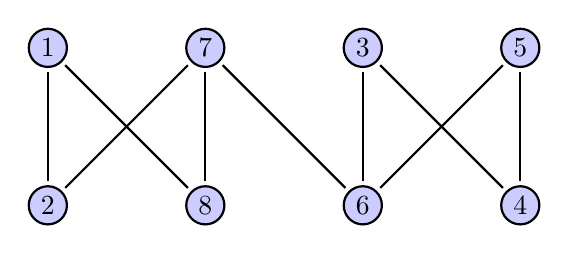
\begin{tikzpicture}[node distance=0.5cm,
                       thick,main node/.style={circle,fill=blue!20,draw,outer sep=2pt,inner sep=2pt}
                      ] 
                       \node[main node] (1) at (-3.00,2.00) {$1$};
  \node[main node] (7) at (-1.00,2.00) {$7$};
  \node[main node] (3) at (1.00,2.00) {$3$};
  \node[main node] (5) at (3.00,2.00) {$5$};
  \node[main node] (4) at (3.00,0.00) {$4$};
  \node[main node] (6) at (1.00,0.00) {$6$};
  \node[main node] (8) at (-1.00,0.00) {$8$};
  \node[main node] (2) at (-3.00,0.00) {$2$};

  \path%
   (1) edge [left] node {} (2)
   (3) edge [left] node {} (4)
   (1) edge [left] node {} (8)
   (2) edge [left] node {} (7)
   (3) edge [left] node {} (6)
   (4) edge [left] node {} (5)
   (8) edge [left] node {} (7)
   (7) edge [left] node {} (6)
   (6) edge [left] node {} (5);
 \end{tikzpicture}
\end{Solution}

    
\begin{Solution}{38.4}
A hamiltonian circuit is $a,b,c,d,e,f,g,h,i,j,a$.

The graph $G$ has four vertices of odd degree, so it is not eulerian.

\end{Solution}

    
\begin{Solution}{38.5}

An euler circuit is $a,b,c,d,e,f,g,h,a,d,g,b,e,h,c,f,a$.

\end{Solution}

    
\begin{Solution}{38.6}

In a hamiltonian circuit, exactly two edges must be used at each vertex. Therefore a hamiltonian circuit would include the edges $\{a,b\}, \{a,j\}, \{b,c\}, \{c,d\}, \{d,g\},$ and $\{g,h\}$. But then the edges $\{b,i\}, \{b,e\},$ and
$\{e,d\}$ would be forbidden. This leave only the single edge $\{e,f\}$ to include $e$ in the circuit. Conclusion: the graph  $G$ is not hamiltonian. 

\end{Solution}

